% appendix/questions/time.tex
% SPDX-License-Identifier: CC-BY-SA-3.0

\section{What Time Is It?}
\label{sec:app:questions:What Time Is It?}

\begin{figure}[htb]
\centering
\resizebox{2.6in}{!}{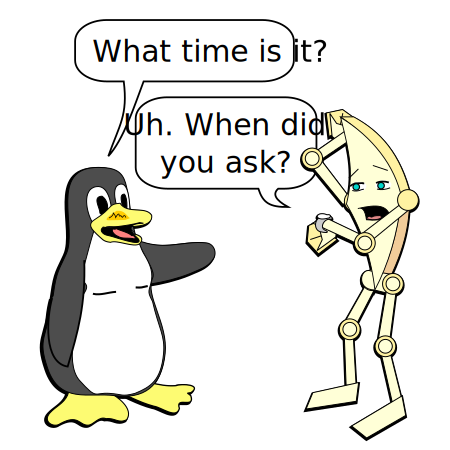
\includegraphics{cartoons/r-2014-What-time-is-it}}
\caption{What Time Is It?}
\ContributedBy{Figure}{fig:app:questions:What Time Is It?}{Melissa Broussard}
\end{figure}

멀티코어 컴퓨터에서 시간을 관리하는데 있어서의 핵심 문제가
Figure~\ref{fig:app:questions:What Time Is It?} 에 그려져 있습니다.
한가지 문제는 시간을 읽는데에도 시간이 걸린다는 점입니다.
하나의 인스트럭션을 통해 하드웨어 시계를 읽을 것이고, 이 읽기 오퍼레이션을
완료하기 위해서 코어 바깥으로 (더 나쁜 경우라면, socket 바깥으로) 나가야 할
겁니다.
또한, 읽어온 값에 대해서 어떤 계산을 해야할 수도 있는데, 예를 들어, 요구된
형태로 변환을 하기 위해, 또는 네트워크 타임 프로토콜 (NTP) 을 통한 조정을
가하기 위해, 등등의 이유로 인해서입니다.
그러니 최종적으로 리턴되는 시간은, 시간을 얻어도기 위해 걸린 시간의
시작점에서의 시각일까요, 끝에서의 시각일까요, 또는 그사이 어딘가일까요?

더 나쁜건, 시간을 읽는 쓰레드가 인터럽트 당하거나 preemption 당할 수도
있습니다.
더 나아가서, 시간을 읽어오고 나서 실제로 그렇게 읽어온 시간을 사용하기 전에
또다른 계산 과정이 들어갈 수도 있습니다.
이런 가능성들이 불확실한 시간 간격을 더 늘립니다.
\iffalse

A key issue with timekeeping on multicore computer systems is illustrated
by Figure~\ref{fig:app:questions:What Time Is It?}.
One problem is that it takes time to read out the time.
An instruction might read from a hardware clock, and might
have to go off-core (or worse yet, off-socket) to complete
this read operation.
It might also be necessary to do some computation on the value read out,
for example, to convert it to the desired format, to apply network time
protocol (NTP) adjustments, and so on.
So does the time eventually returned correspond to the beginning of
the resulting time interval, the end, or somewhere in between?

Worse yet, the thread reading the time might be interrupted or preempted.
Furthermore, there will likely be some computation between reading out
the time and the actual use of the time that has been read out.
Both of these possibilities further extend the interval of uncertainty.
\fi

이에 대한 한가지 방법은 시간을 두번 읽고, 이렇게 읽어온 두가지 값의 평균을
사용하는 것입니다.
두번의 읽어온 값 사이의 차이는 사이에 낀 오퍼레이션이 발생시킨 시간의
불확실성의 정도입니다.

물론, 많은 경우에, 정확한 시각이 필요치는 않습니다.
예를 들어, 사람이 사용하기 위한 시각을 프린트 하는 경우에 있어서는, 우리는 내부
하드웨어와 소프트웨어의 비규칙적인 딜레이를 처리하는데에 있어, 사람의 느린
반응성에 의존할 수 있습니다.
비슷하게, 어떤 서버가 클라이언트로의 응답 시간을 측정해야 한다면, 요청의 도착
시각과 응답의 전송 사이의 시각은 똑같이 괜찮을 겁니다.
\iffalse

One approach is to read the time twice, and take the arithmetic mean
of the two readings, perhaps one on each side of the operation being
timestamped.
The difference between the two readings is then a measure of uncertainty
of the time at which the intervening operation occurred.

Of course, in many cases, the exact time is not necessary.
For example, when printing the time for the benefit of a human user,
we can rely on slow human reflexes to render internal hardware and
software delays irrelevant.
Similarly, if a server needs to timestamp the response to a client, any
time between the reception of the request and the transmission of the
response will do equally well.
\fi

% @@@ Scheduling ticks

% @@@ Tickless operation

% @@@ Timers

% @@@ Current time, monotonic operation

% @@@ The many ways in which time can appear to go backwards

% @@@ Causality, the only real time in SMP (or distributed) systems
